\documentclass[a4paper]{book}
\usepackage{makeidx}
\usepackage{graphicx}
\usepackage{multicol}
\usepackage{float}
\usepackage{listings}
\usepackage{color}
\usepackage{textcomp}
\usepackage{alltt}
\usepackage{times}
\usepackage{ifpdf}
\ifpdf
\usepackage[pdftex,
            pagebackref=true,
            colorlinks=true,
            linkcolor=blue,
            unicode
           ]{hyperref}
\else
\usepackage[ps2pdf,
            pagebackref=true,
            colorlinks=true,
            linkcolor=blue,
            unicode
           ]{hyperref}
\usepackage{pspicture}
\fi
\usepackage[utf8]{inputenc}
\usepackage{polski}
\usepackage[T1]{fontenc}

\usepackage{doxygen}
\lstset{language=C++,inputencoding=utf8,basicstyle=\footnotesize,breaklines=true,breakatwhitespace=true,tabsize=4,numbers=left }
\makeindex
\setcounter{tocdepth}{3}
\renewcommand{\footrulewidth}{0.4pt}
\begin{document}
\hypersetup{pageanchor=false}
\begin{titlepage}
\vspace*{7cm}
\begin{center}
{\Large Struktury\_\-Tablice\_\-Dynamiczne \\[1ex]\large 1 }\\
\vspace*{1cm}
{\large Wygenerowano przez Doxygen 1.7.1}\\
\vspace*{0.5cm}
{\small Thu Mar 26 2015 06:32:47}\\
\end{center}
\end{titlepage}
\clearemptydoublepage
\pagenumbering{roman}
\tableofcontents
\clearemptydoublepage
\pagenumbering{arabic}
\hypersetup{pageanchor=true}
\chapter{Program tworzacy struktury danych.}
\label{index}\hypertarget{index}{}\begin{DoxyAuthor}{Autor}
Lukasz Sak 
\end{DoxyAuthor}
\begin{DoxyVersion}{Wersja}
1
\end{DoxyVersion}
Program posiada definicje struktur danych: \hyperlink{class_stos}{Stos}, \hyperlink{class_lista}{Lista}, \hyperlink{class_kolejka}{Kolejka}. Struktury posiadaja wiekszosc takich samych metod. PUSH() -\/ wrzucajaca dana do struktury, POP() -\/ usuwajacy odpowiednia dana ze struktury, SIZE() -\/ zwracajacy ilosc elementow w strukturze, SHOW() -\/ wyswietlajacy elementy struktury. Struktury sa zrobione na szablonach, zatem mozna uzywac kilku typow danych. 
\chapter{Indeks klas}
\section{Hierarchia klas}
Ta lista dziedziczenia posortowana jest z grubsza, choć nie całkowicie, alfabetycznie:\begin{DoxyCompactList}
\item \contentsline{section}{Benchmark}{\pageref{class_benchmark}}{}
\item \contentsline{section}{Lista$<$ TYP $>$}{\pageref{class_lista}}{}
\begin{DoxyCompactList}
\item \contentsline{section}{Kolejka$<$ TYP $>$}{\pageref{class_kolejka}}{}
\item \contentsline{section}{Stos$<$ TYP $>$}{\pageref{class_stos}}{}
\end{DoxyCompactList}
\end{DoxyCompactList}

\chapter{Indeks klas}
\section{Lista klas}
Tutaj znajdują się klasy, struktury, unie i interfejsy wraz z ich krótkimi opisami:\begin{DoxyCompactList}
\item\contentsline{section}{\hyperlink{class_benchmark}{Benchmark} (Klasa \hyperlink{class_benchmark}{Benchmark} )}{\pageref{class_benchmark}}{}
\item\contentsline{section}{\hyperlink{class_kolejka}{Kolejka$<$ TYP $>$} (Klasa \hyperlink{class_kolejka}{Kolejka} )}{\pageref{class_kolejka}}{}
\item\contentsline{section}{\hyperlink{class_lista}{Lista$<$ TYP $>$} (Klasa \hyperlink{class_lista}{Lista} )}{\pageref{class_lista}}{}
\item\contentsline{section}{\hyperlink{class_stos}{Stos$<$ TYP $>$} (Klasa \hyperlink{class_stos}{Stos} )}{\pageref{class_stos}}{}
\end{DoxyCompactList}

\chapter{Indeks plików}
\section{Lista plików}
Tutaj znajduje się lista wszystkich plików z ich krótkimi opisami:\begin{DoxyCompactList}
\item\contentsline{section}{\hyperlink{_benchmark_8cpp}{Benchmark.cpp} (Metody klasy \hyperlink{class_benchmark}{Benchmark} )}{\pageref{_benchmark_8cpp}}{}
\item\contentsline{section}{\hyperlink{_benchmark_8hh}{Benchmark.hh} (Definicja klasy \hyperlink{class_benchmark}{Benchmark} )}{\pageref{_benchmark_8hh}}{}
\item\contentsline{section}{\hyperlink{_element_8hh}{Element.hh} (Definicja klasy \hyperlink{class_element}{Element} )}{\pageref{_element_8hh}}{}
\item\contentsline{section}{\hyperlink{_kolejka_8hh}{Kolejka.hh} (Definicja klasy \hyperlink{class_kolejka}{Kolejka} )}{\pageref{_kolejka_8hh}}{}
\item\contentsline{section}{\hyperlink{_lista_8hh}{Lista.hh} (Definicja klasy \hyperlink{class_lista}{Lista} )}{\pageref{_lista_8hh}}{}
\item\contentsline{section}{\hyperlink{_stos_8hh}{Stos.hh} (Definicja klasy \hyperlink{class_stos}{Stos} )}{\pageref{_stos_8hh}}{}
\item\contentsline{section}{\hyperlink{_struktury_8cpp}{Struktury.cpp} }{\pageref{_struktury_8cpp}}{}
\item\contentsline{section}{\hyperlink{_test_8cpp}{Test.cpp} }{\pageref{_test_8cpp}}{}
\end{DoxyCompactList}

\chapter{Dokumentacja klas}
\hypertarget{class_benchmark}{
\section{Dokumentacja klasy Benchmark}
\label{class_benchmark}\index{Benchmark@{Benchmark}}
}


Klasa \hyperlink{class_benchmark}{Benchmark}.  




{\ttfamily \#include $<$Benchmark.hh$>$}

\subsection*{Metody publiczne}
\begin{DoxyCompactItemize}
\item 
\hyperlink{class_benchmark_a0d31c546243991bb9a740494dce9b2b1}{Benchmark} (unsigned int rozmiar\_\-problemu, double stala)
\begin{DoxyCompactList}\small\item\em Inicjalizator klasy \hyperlink{class_benchmark}{Benchmark}. \item\end{DoxyCompactList}\item 
double \hyperlink{class_benchmark_a15630af66f064ee79928ae58f74c87c0}{Tablica} (int i)
\item 
float \hyperlink{class_benchmark_a099a0e33f94c72bdc90006cd88bae3d7}{Licz\_\-Srednia} ()
\item 
float \hyperlink{class_benchmark_a52f1076c0e71389f8c962380e5354fed}{Czas\_\-Start} ()
\item 
float \hyperlink{class_benchmark_a178ddfabb8289612748453ecf0bfd600}{Czas\_\-Stop} ()
\item 
void \hyperlink{class_benchmark_a6b8ee09e9e44c458c007d27105463085}{Zapisz\_\-Wyniki} ()
\item 
\hyperlink{class_benchmark_a20476e07f09e2b20ed3e9a7f13a570e6}{$\sim$Benchmark} ()
\end{DoxyCompactItemize}
\subsection*{Atrybuty publiczne}
\begin{DoxyCompactItemize}
\item 
unsigned int $\ast$ \hyperlink{class_benchmark_aef4c89962e86bfe41f406c620e4b6ec6}{wielkosc\_\-problemu}
\item 
unsigned int \hyperlink{class_benchmark_a5f29a9983dd88241a17c4a9b2a86e9e1}{Ilosc\_\-Danych}
\end{DoxyCompactItemize}
\subsection*{Metody prywatne}
\begin{DoxyCompactItemize}
\item 
void \hyperlink{class_benchmark_a105f31cf198d96969b939e7bacaa9354}{Losuj} (int $\ast$tablica\_\-liczb, unsigned int rozmiar)
\item 
unsigned int \hyperlink{class_benchmark_aa514b55bb3d7c5eb4c1862dbdbc313b6}{Wczytaj\_\-Dane} ()
\end{DoxyCompactItemize}
\subsection*{Atrybuty prywatne}
\begin{DoxyCompactItemize}
\item 
int $\ast$ \hyperlink{class_benchmark_af550349e9f512c47bd5f4fd6f0630913}{\_\-tablica\_\-liczb}
\item 
float \hyperlink{class_benchmark_a9809e00b248161927de3cbd71fd8d424}{stoper\_\-start}
\item 
unsigned int \hyperlink{class_benchmark_ae1cbaa987a9ac13bc40dbe4b84a587b6}{iterator}
\item 
unsigned int \hyperlink{class_benchmark_a12925bcca68de983919ebd5d6b9e2b01}{iterator\_\-sredniej}
\item 
float $\ast$ \hyperlink{class_benchmark_aa33949783712cd5f501a32b4f497f8e9}{stoper\_\-stop}
\item 
float $\ast$ \hyperlink{class_benchmark_a1eea18c08dc325a4723ef0b2084938d6}{srednia\_\-jednego\_\-problemu}
\item 
unsigned int \hyperlink{class_benchmark_a30d4c478ec859f45df0ac80ac1a89203}{rozmiar\_\-tablic}
\end{DoxyCompactItemize}


\subsection{Opis szczegółowy}
Klasa ta modeluje nam test dla funkcji Składa się z pól: 
\begin{DoxyParams}{Parametry}
\item[\mbox{\tt[in]} {\em \_\-tablica\_\-liczb}]-\/ która przechowuje nasze dane ktorymi bedziemy testowali funkcje \item[\mbox{\tt[in]} {\em stoper\_\-start}]-\/ przechowuje poczatek mierzenia czasu \item[\mbox{\tt[in]} {\em iterator}]-\/ sluzy nam do iterowania od 0 do 9 (10 prob) zatrzymania czasu \item[\mbox{\tt[in]} {\em iterator\_\-sredniej}]-\/ sluzy nam do iterowania kolejnego pomiaru sredniej w zaleznosci od ilosci prob \item[\mbox{\tt[in]} {\em stoper\_\-stop}]-\/ przechowuje nam 10 wynikow pomiaru czasu (obliczony wynik jednego pomiaru) \item[\mbox{\tt[in]} {\em srednia\_\-jednego\_\-problemu}]-\/ przechowuje tablice sredniego czasu wykonania pomiarow dla poszczegolnych prob \item[\mbox{\tt[in]} {\em ilosc\_\-problemu}]-\/ przechowuje nam jak duzo prob bedzie wykonywanych \item[\mbox{\tt[in]} {\em Ilosc\_\-Danych}]-\/ ilosc danych na ktorych bedziemy pracowali \item[\mbox{\tt[in]} {\em wielkosc\_\-problemu}]-\/ ilosc pojedynczego problemu(ilosci danych na 1 probe) \end{DoxyParams}


Definicja w linii 30 pliku Benchmark.hh.



\subsection{Dokumentacja konstruktora i destruktora}
\hypertarget{class_benchmark_a0d31c546243991bb9a740494dce9b2b1}{
\index{Benchmark@{Benchmark}!Benchmark@{Benchmark}}
\index{Benchmark@{Benchmark}!Benchmark@{Benchmark}}
\subsubsection[{Benchmark}]{\setlength{\rightskip}{0pt plus 5cm}Benchmark::Benchmark (
\begin{DoxyParamCaption}
\item[{unsigned int}]{ rozmiar\_\-problemu, }
\item[{double}]{ stala}
\end{DoxyParamCaption}
)}}
\label{class_benchmark_a0d31c546243991bb9a740494dce9b2b1}
Inicjalizator ten służy do określania początkowych wartości pól klasy oraz wyboru na jakich danych bedziemy pracowali (losowe/wczytane)

Opis argumentów: 
\begin{DoxyParams}{Parametry}
\item[\mbox{\tt[in]} {\em rozmiar\_\-problemu}]-\/ ilosc maksymalnej liczby wprowadzanych danych \item[\mbox{\tt[in]} {\em stala}]-\/ stala przez ktora bedziemy mnozyli, aby np.uzyskac wiecej wynikow najlepszy przedzial (1.1-\/10) \end{DoxyParams}


Definicja w linii 15 pliku Benchmark.cpp.



Oto graf wywołań dla tej funkcji:
\nopagebreak
\begin{figure}[H]
\begin{center}
\leavevmode
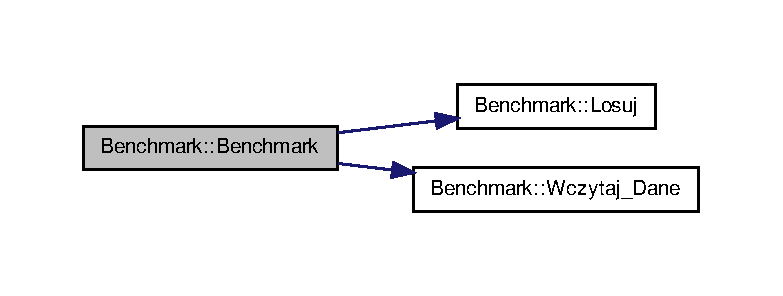
\includegraphics[width=376pt]{class_benchmark_a0d31c546243991bb9a740494dce9b2b1_cgraph}
\end{center}
\end{figure}


\hypertarget{class_benchmark_a20476e07f09e2b20ed3e9a7f13a570e6}{
\index{Benchmark@{Benchmark}!$\sim$Benchmark@{$\sim$Benchmark}}
\index{$\sim$Benchmark@{$\sim$Benchmark}!Benchmark@{Benchmark}}
\subsubsection[{$\sim$Benchmark}]{\setlength{\rightskip}{0pt plus 5cm}Benchmark::$\sim$Benchmark (
\begin{DoxyParamCaption}
{}
\end{DoxyParamCaption}
)\hspace{0.3cm}{\ttfamily  \mbox{[}inline\mbox{]}}}}
\label{class_benchmark_a20476e07f09e2b20ed3e9a7f13a570e6}


Definicja w linii 125 pliku Benchmark.hh.



\subsection{Dokumentacja funkcji składowych}
\hypertarget{class_benchmark_a52f1076c0e71389f8c962380e5354fed}{
\index{Benchmark@{Benchmark}!Czas\_\-Start@{Czas\_\-Start}}
\index{Czas\_\-Start@{Czas\_\-Start}!Benchmark@{Benchmark}}
\subsubsection[{Czas\_\-Start}]{\setlength{\rightskip}{0pt plus 5cm}float Benchmark::Czas\_\-Start (
\begin{DoxyParamCaption}
{}
\end{DoxyParamCaption}
)}}
\label{class_benchmark_a52f1076c0e71389f8c962380e5354fed}


Definicja w linii 66 pliku Benchmark.cpp.



Oto graf wywoływań tej funkcji:
\nopagebreak
\begin{figure}[H]
\begin{center}
\leavevmode
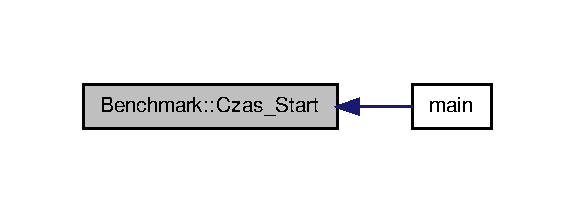
\includegraphics[width=276pt]{class_benchmark_a52f1076c0e71389f8c962380e5354fed_icgraph}
\end{center}
\end{figure}


\hypertarget{class_benchmark_a178ddfabb8289612748453ecf0bfd600}{
\index{Benchmark@{Benchmark}!Czas\_\-Stop@{Czas\_\-Stop}}
\index{Czas\_\-Stop@{Czas\_\-Stop}!Benchmark@{Benchmark}}
\subsubsection[{Czas\_\-Stop}]{\setlength{\rightskip}{0pt plus 5cm}float Benchmark::Czas\_\-Stop (
\begin{DoxyParamCaption}
{}
\end{DoxyParamCaption}
)}}
\label{class_benchmark_a178ddfabb8289612748453ecf0bfd600}


Definicja w linii 73 pliku Benchmark.cpp.



Oto graf wywoływań tej funkcji:
\nopagebreak
\begin{figure}[H]
\begin{center}
\leavevmode
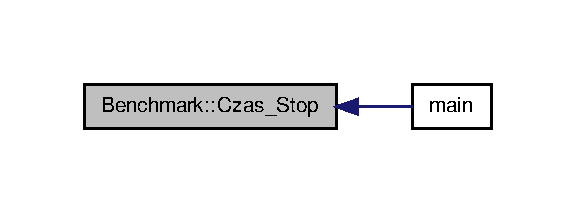
\includegraphics[width=276pt]{class_benchmark_a178ddfabb8289612748453ecf0bfd600_icgraph}
\end{center}
\end{figure}


\hypertarget{class_benchmark_a099a0e33f94c72bdc90006cd88bae3d7}{
\index{Benchmark@{Benchmark}!Licz\_\-Srednia@{Licz\_\-Srednia}}
\index{Licz\_\-Srednia@{Licz\_\-Srednia}!Benchmark@{Benchmark}}
\subsubsection[{Licz\_\-Srednia}]{\setlength{\rightskip}{0pt plus 5cm}float Benchmark::Licz\_\-Srednia (
\begin{DoxyParamCaption}
{}
\end{DoxyParamCaption}
)}}
\label{class_benchmark_a099a0e33f94c72bdc90006cd88bae3d7}


Definicja w linii 83 pliku Benchmark.cpp.



Oto graf wywoływań tej funkcji:
\nopagebreak
\begin{figure}[H]
\begin{center}
\leavevmode
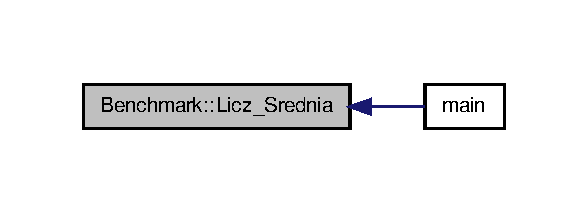
\includegraphics[width=282pt]{class_benchmark_a099a0e33f94c72bdc90006cd88bae3d7_icgraph}
\end{center}
\end{figure}


\hypertarget{class_benchmark_a105f31cf198d96969b939e7bacaa9354}{
\index{Benchmark@{Benchmark}!Losuj@{Losuj}}
\index{Losuj@{Losuj}!Benchmark@{Benchmark}}
\subsubsection[{Losuj}]{\setlength{\rightskip}{0pt plus 5cm}void Benchmark::Losuj (
\begin{DoxyParamCaption}
\item[{int $\ast$}]{ tablica\_\-liczb, }
\item[{unsigned int}]{ rozmiar}
\end{DoxyParamCaption}
)\hspace{0.3cm}{\ttfamily  \mbox{[}private\mbox{]}}}}
\label{class_benchmark_a105f31cf198d96969b939e7bacaa9354}


Definicja w linii 56 pliku Benchmark.cpp.



Oto graf wywoływań tej funkcji:
\nopagebreak
\begin{figure}[H]
\begin{center}
\leavevmode
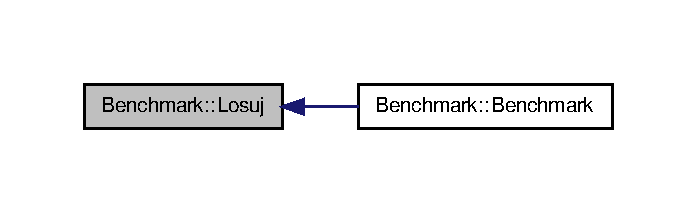
\includegraphics[width=334pt]{class_benchmark_a105f31cf198d96969b939e7bacaa9354_icgraph}
\end{center}
\end{figure}


\hypertarget{class_benchmark_a15630af66f064ee79928ae58f74c87c0}{
\index{Benchmark@{Benchmark}!Tablica@{Tablica}}
\index{Tablica@{Tablica}!Benchmark@{Benchmark}}
\subsubsection[{Tablica}]{\setlength{\rightskip}{0pt plus 5cm}double Benchmark::Tablica (
\begin{DoxyParamCaption}
\item[{int}]{ i}
\end{DoxyParamCaption}
)\hspace{0.3cm}{\ttfamily  \mbox{[}inline\mbox{]}}}}
\label{class_benchmark_a15630af66f064ee79928ae58f74c87c0}


Definicja w linii 83 pliku Benchmark.hh.



Oto graf wywoływań tej funkcji:
\nopagebreak
\begin{figure}[H]
\begin{center}
\leavevmode
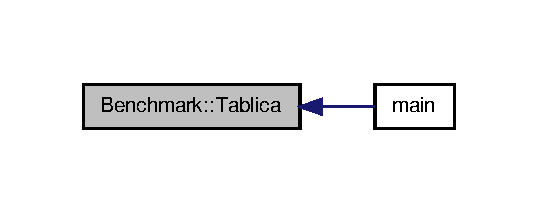
\includegraphics[width=258pt]{class_benchmark_a15630af66f064ee79928ae58f74c87c0_icgraph}
\end{center}
\end{figure}


\hypertarget{class_benchmark_aa514b55bb3d7c5eb4c1862dbdbc313b6}{
\index{Benchmark@{Benchmark}!Wczytaj\_\-Dane@{Wczytaj\_\-Dane}}
\index{Wczytaj\_\-Dane@{Wczytaj\_\-Dane}!Benchmark@{Benchmark}}
\subsubsection[{Wczytaj\_\-Dane}]{\setlength{\rightskip}{0pt plus 5cm}unsigned int Benchmark::Wczytaj\_\-Dane (
\begin{DoxyParamCaption}
{}
\end{DoxyParamCaption}
)\hspace{0.3cm}{\ttfamily  \mbox{[}private\mbox{]}}}}
\label{class_benchmark_aa514b55bb3d7c5eb4c1862dbdbc313b6}


Definicja w linii 114 pliku Benchmark.cpp.



Oto graf wywoływań tej funkcji:
\nopagebreak
\begin{figure}[H]
\begin{center}
\leavevmode
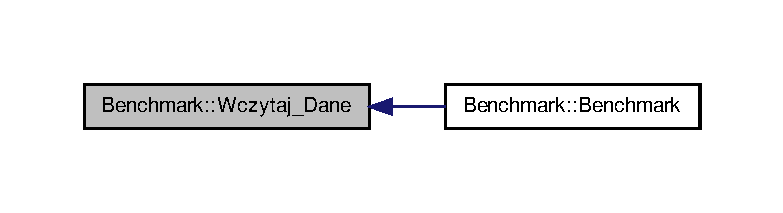
\includegraphics[width=376pt]{class_benchmark_aa514b55bb3d7c5eb4c1862dbdbc313b6_icgraph}
\end{center}
\end{figure}


\hypertarget{class_benchmark_a6b8ee09e9e44c458c007d27105463085}{
\index{Benchmark@{Benchmark}!Zapisz\_\-Wyniki@{Zapisz\_\-Wyniki}}
\index{Zapisz\_\-Wyniki@{Zapisz\_\-Wyniki}!Benchmark@{Benchmark}}
\subsubsection[{Zapisz\_\-Wyniki}]{\setlength{\rightskip}{0pt plus 5cm}void Benchmark::Zapisz\_\-Wyniki (
\begin{DoxyParamCaption}
{}
\end{DoxyParamCaption}
)}}
\label{class_benchmark_a6b8ee09e9e44c458c007d27105463085}


Definicja w linii 95 pliku Benchmark.cpp.



Oto graf wywoływań tej funkcji:
\nopagebreak
\begin{figure}[H]
\begin{center}
\leavevmode
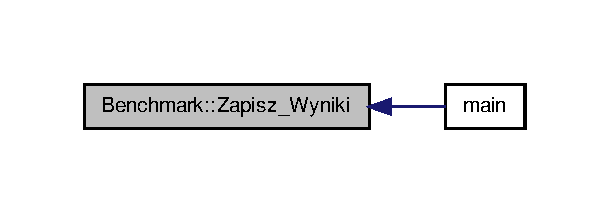
\includegraphics[width=292pt]{class_benchmark_a6b8ee09e9e44c458c007d27105463085_icgraph}
\end{center}
\end{figure}




\subsection{Dokumentacja atrybutów składowych}
\hypertarget{class_benchmark_af550349e9f512c47bd5f4fd6f0630913}{
\index{Benchmark@{Benchmark}!\_\-tablica\_\-liczb@{\_\-tablica\_\-liczb}}
\index{\_\-tablica\_\-liczb@{\_\-tablica\_\-liczb}!Benchmark@{Benchmark}}
\subsubsection[{\_\-tablica\_\-liczb}]{\setlength{\rightskip}{0pt plus 5cm}int$\ast$ {\bf Benchmark::\_\-tablica\_\-liczb}\hspace{0.3cm}{\ttfamily  \mbox{[}private\mbox{]}}}}
\label{class_benchmark_af550349e9f512c47bd5f4fd6f0630913}


Definicja w linii 32 pliku Benchmark.hh.

\hypertarget{class_benchmark_a5f29a9983dd88241a17c4a9b2a86e9e1}{
\index{Benchmark@{Benchmark}!Ilosc\_\-Danych@{Ilosc\_\-Danych}}
\index{Ilosc\_\-Danych@{Ilosc\_\-Danych}!Benchmark@{Benchmark}}
\subsubsection[{Ilosc\_\-Danych}]{\setlength{\rightskip}{0pt plus 5cm}unsigned int {\bf Benchmark::Ilosc\_\-Danych}}}
\label{class_benchmark_a5f29a9983dd88241a17c4a9b2a86e9e1}


Definicja w linii 74 pliku Benchmark.hh.

\hypertarget{class_benchmark_ae1cbaa987a9ac13bc40dbe4b84a587b6}{
\index{Benchmark@{Benchmark}!iterator@{iterator}}
\index{iterator@{iterator}!Benchmark@{Benchmark}}
\subsubsection[{iterator}]{\setlength{\rightskip}{0pt plus 5cm}unsigned int {\bf Benchmark::iterator}\hspace{0.3cm}{\ttfamily  \mbox{[}private\mbox{]}}}}
\label{class_benchmark_ae1cbaa987a9ac13bc40dbe4b84a587b6}


Definicja w linii 34 pliku Benchmark.hh.

\hypertarget{class_benchmark_a12925bcca68de983919ebd5d6b9e2b01}{
\index{Benchmark@{Benchmark}!iterator\_\-sredniej@{iterator\_\-sredniej}}
\index{iterator\_\-sredniej@{iterator\_\-sredniej}!Benchmark@{Benchmark}}
\subsubsection[{iterator\_\-sredniej}]{\setlength{\rightskip}{0pt plus 5cm}unsigned int {\bf Benchmark::iterator\_\-sredniej}\hspace{0.3cm}{\ttfamily  \mbox{[}private\mbox{]}}}}
\label{class_benchmark_a12925bcca68de983919ebd5d6b9e2b01}


Definicja w linii 35 pliku Benchmark.hh.

\hypertarget{class_benchmark_a30d4c478ec859f45df0ac80ac1a89203}{
\index{Benchmark@{Benchmark}!rozmiar\_\-tablic@{rozmiar\_\-tablic}}
\index{rozmiar\_\-tablic@{rozmiar\_\-tablic}!Benchmark@{Benchmark}}
\subsubsection[{rozmiar\_\-tablic}]{\setlength{\rightskip}{0pt plus 5cm}unsigned int {\bf Benchmark::rozmiar\_\-tablic}\hspace{0.3cm}{\ttfamily  \mbox{[}private\mbox{]}}}}
\label{class_benchmark_a30d4c478ec859f45df0ac80ac1a89203}


Definicja w linii 38 pliku Benchmark.hh.

\hypertarget{class_benchmark_a1eea18c08dc325a4723ef0b2084938d6}{
\index{Benchmark@{Benchmark}!srednia\_\-jednego\_\-problemu@{srednia\_\-jednego\_\-problemu}}
\index{srednia\_\-jednego\_\-problemu@{srednia\_\-jednego\_\-problemu}!Benchmark@{Benchmark}}
\subsubsection[{srednia\_\-jednego\_\-problemu}]{\setlength{\rightskip}{0pt plus 5cm}float$\ast$ {\bf Benchmark::srednia\_\-jednego\_\-problemu}\hspace{0.3cm}{\ttfamily  \mbox{[}private\mbox{]}}}}
\label{class_benchmark_a1eea18c08dc325a4723ef0b2084938d6}


Definicja w linii 37 pliku Benchmark.hh.

\hypertarget{class_benchmark_a9809e00b248161927de3cbd71fd8d424}{
\index{Benchmark@{Benchmark}!stoper\_\-start@{stoper\_\-start}}
\index{stoper\_\-start@{stoper\_\-start}!Benchmark@{Benchmark}}
\subsubsection[{stoper\_\-start}]{\setlength{\rightskip}{0pt plus 5cm}float {\bf Benchmark::stoper\_\-start}\hspace{0.3cm}{\ttfamily  \mbox{[}private\mbox{]}}}}
\label{class_benchmark_a9809e00b248161927de3cbd71fd8d424}


Definicja w linii 33 pliku Benchmark.hh.

\hypertarget{class_benchmark_aa33949783712cd5f501a32b4f497f8e9}{
\index{Benchmark@{Benchmark}!stoper\_\-stop@{stoper\_\-stop}}
\index{stoper\_\-stop@{stoper\_\-stop}!Benchmark@{Benchmark}}
\subsubsection[{stoper\_\-stop}]{\setlength{\rightskip}{0pt plus 5cm}float$\ast$ {\bf Benchmark::stoper\_\-stop}\hspace{0.3cm}{\ttfamily  \mbox{[}private\mbox{]}}}}
\label{class_benchmark_aa33949783712cd5f501a32b4f497f8e9}


Definicja w linii 36 pliku Benchmark.hh.

\hypertarget{class_benchmark_aef4c89962e86bfe41f406c620e4b6ec6}{
\index{Benchmark@{Benchmark}!wielkosc\_\-problemu@{wielkosc\_\-problemu}}
\index{wielkosc\_\-problemu@{wielkosc\_\-problemu}!Benchmark@{Benchmark}}
\subsubsection[{wielkosc\_\-problemu}]{\setlength{\rightskip}{0pt plus 5cm}unsigned int$\ast$ {\bf Benchmark::wielkosc\_\-problemu}}}
\label{class_benchmark_aef4c89962e86bfe41f406c620e4b6ec6}


Definicja w linii 73 pliku Benchmark.hh.



Dokumentacja dla tej klasy została wygenerowana z plików:\begin{DoxyCompactItemize}
\item 
\hyperlink{_benchmark_8hh}{Benchmark.hh}\item 
\hyperlink{_benchmark_8cpp}{Benchmark.cpp}\end{DoxyCompactItemize}

\hypertarget{class_kolejka}{
\section{Dokumentacja szablonu klasy Kolejka$<$ TYP $>$}
\label{class_kolejka}\index{Kolejka@{Kolejka}}
}


Klasa \hyperlink{class_kolejka}{Kolejka}.  




{\ttfamily \#include $<$Kolejka.hh$>$}



Diagram dziedziczenia dla Kolejka$<$ TYP $>$
\nopagebreak
\begin{figure}[H]
\begin{center}
\leavevmode
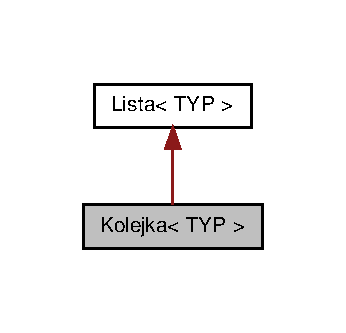
\includegraphics[width=166pt]{class_kolejka__inherit__graph}
\end{center}
\end{figure}


Diagram współpracy dla Kolejka$<$ TYP $>$:
\nopagebreak
\begin{figure}[H]
\begin{center}
\leavevmode
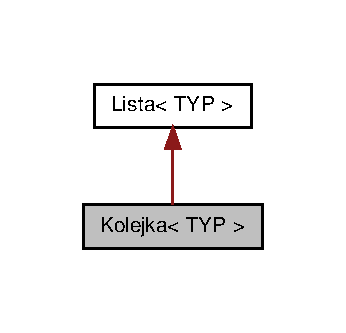
\includegraphics[width=166pt]{class_kolejka__coll__graph}
\end{center}
\end{figure}
\subsection*{Metody publiczne}
\begin{DoxyCompactItemize}
\item 
void \hyperlink{class_kolejka_a66056e67a0514466d7771da351e8468b}{PUSH} (TYP liczba)
\item 
int \hyperlink{class_kolejka_ab1d8e5d4a855fb2156201a57cc0a9a39}{POP} ()
\item 
void \hyperlink{class_kolejka_a26b5afbcc9f892a41acbd3aed062ee50}{SHOW} ()
\item 
unsigned int \hyperlink{class_kolejka_a06a7fe157ff434771a700ffd084dc7a2}{SIZE} ()
\end{DoxyCompactItemize}


\subsection{Opis szczegółowy}
\subsubsection*{template$<$typename TYP$>$ class Kolejka$<$ TYP $>$}

Klasa ta modeluje nam Kolejke Składa się z pól klasy \hyperlink{class_lista}{Lista} (poczatek) oraz metod PUSH, POP, SIZE, SHOW Klasa w calosci wykorzystuje implementacje listy 

Definicja w linii 25 pliku Kolejka.hh.



\subsection{Dokumentacja funkcji składowych}
\hypertarget{class_kolejka_ab1d8e5d4a855fb2156201a57cc0a9a39}{
\index{Kolejka@{Kolejka}!POP@{POP}}
\index{POP@{POP}!Kolejka@{Kolejka}}
\subsubsection[{POP}]{\setlength{\rightskip}{0pt plus 5cm}template$<$typename TYP $>$ int {\bf Kolejka}$<$ TYP $>$::POP (
\begin{DoxyParamCaption}
{}
\end{DoxyParamCaption}
)\hspace{0.3cm}{\ttfamily  \mbox{[}inline\mbox{]}}}}
\label{class_kolejka_ab1d8e5d4a855fb2156201a57cc0a9a39}


Definicja w linii 41 pliku Kolejka.hh.

\hypertarget{class_kolejka_a66056e67a0514466d7771da351e8468b}{
\index{Kolejka@{Kolejka}!PUSH@{PUSH}}
\index{PUSH@{PUSH}!Kolejka@{Kolejka}}
\subsubsection[{PUSH}]{\setlength{\rightskip}{0pt plus 5cm}template$<$typename TYP $>$ void {\bf Kolejka}$<$ TYP $>$::PUSH (
\begin{DoxyParamCaption}
\item[{TYP}]{ liczba}
\end{DoxyParamCaption}
)\hspace{0.3cm}{\ttfamily  \mbox{[}inline\mbox{]}}}}
\label{class_kolejka_a66056e67a0514466d7771da351e8468b}


Reimplementowana z \hyperlink{class_lista_a5c21bab22b627c729ad0c90e1f835901}{Lista$<$ TYP $>$}.



Definicja w linii 34 pliku Kolejka.hh.

\hypertarget{class_kolejka_a26b5afbcc9f892a41acbd3aed062ee50}{
\index{Kolejka@{Kolejka}!SHOW@{SHOW}}
\index{SHOW@{SHOW}!Kolejka@{Kolejka}}
\subsubsection[{SHOW}]{\setlength{\rightskip}{0pt plus 5cm}template$<$typename TYP $>$ void {\bf Kolejka}$<$ TYP $>$::SHOW (
\begin{DoxyParamCaption}
{}
\end{DoxyParamCaption}
)\hspace{0.3cm}{\ttfamily  \mbox{[}inline\mbox{]}}}}
\label{class_kolejka_a26b5afbcc9f892a41acbd3aed062ee50}


Reimplementowana z \hyperlink{class_lista_a89bbb449a047593eebce602a449ac1e7}{Lista$<$ TYP $>$}.



Definicja w linii 49 pliku Kolejka.hh.

\hypertarget{class_kolejka_a06a7fe157ff434771a700ffd084dc7a2}{
\index{Kolejka@{Kolejka}!SIZE@{SIZE}}
\index{SIZE@{SIZE}!Kolejka@{Kolejka}}
\subsubsection[{SIZE}]{\setlength{\rightskip}{0pt plus 5cm}template$<$typename TYP $>$ unsigned int {\bf Kolejka}$<$ TYP $>$::SIZE (
\begin{DoxyParamCaption}
{}
\end{DoxyParamCaption}
)\hspace{0.3cm}{\ttfamily  \mbox{[}inline\mbox{]}}}}
\label{class_kolejka_a06a7fe157ff434771a700ffd084dc7a2}


Reimplementowana z \hyperlink{class_lista_a4f10ca015c6b34a322dbc1c93e313c07}{Lista$<$ TYP $>$}.



Definicja w linii 58 pliku Kolejka.hh.



Dokumentacja dla tej klasy została wygenerowana z pliku:\begin{DoxyCompactItemize}
\item 
\hyperlink{_kolejka_8hh}{Kolejka.hh}\end{DoxyCompactItemize}

\hypertarget{class_lista}{
\section{Dokumentacja szablonu klasy Lista$<$ TYP $>$}
\label{class_lista}\index{Lista@{Lista}}
}


Klasa \hyperlink{class_lista}{Lista}.  




{\ttfamily \#include $<$Lista.hh$>$}



Diagram dziedziczenia dla Lista$<$ TYP $>$
\nopagebreak
\begin{figure}[H]
\begin{center}
\leavevmode
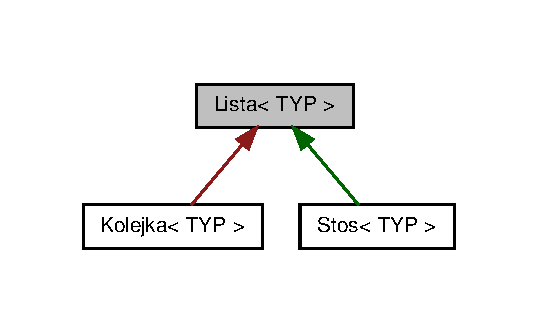
\includegraphics[width=258pt]{class_lista__inherit__graph}
\end{center}
\end{figure}
\subsection*{Metody publiczne}
\begin{DoxyCompactItemize}
\item 
void \hyperlink{class_lista_a81ea74ac702b5ccbe3c88b3149887975}{Rozmiar} ()
\item 
\hyperlink{class_lista_ae2559bf0c96569265d5f9f7f9cd4cb3a}{Lista} ()
\item 
\hyperlink{class_lista_a7271d867e38a838c25ffb5aa6b73faef}{$\sim$Lista} ()
\item 
void \hyperlink{class_lista_a5c21bab22b627c729ad0c90e1f835901}{PUSH} (TYP liczba)
\item 
void \hyperlink{class_lista_a6d81ca560734ac6fce5c503090b7b250}{Powiekszenie\_\-Pamieci} ()
\item 
void \hyperlink{class_lista_aa648e807e5daab59523ffbef5ca80d00}{Zmniejszenie\_\-Pamieci} ()
\item 
int \hyperlink{class_lista_aba90f4f62ac00f38ecf71ba3c9f1b40e}{POP} (int liczba)
\item 
unsigned int \hyperlink{class_lista_a4f10ca015c6b34a322dbc1c93e313c07}{SIZE} ()
\item 
void \hyperlink{class_lista_a89bbb449a047593eebce602a449ac1e7}{SHOW} ()
\end{DoxyCompactItemize}
\subsection*{Atrybuty prywatne}
\begin{DoxyCompactItemize}
\item 
TYP $\ast$ \hyperlink{class_lista_afdd41700bc843ab4aeb58425b63e4390}{tab}
\item 
unsigned int \hyperlink{class_lista_a5d80dd57d8de81690e58a9ee0e33fb68}{\_\-rozmiar\_\-listy}
\item 
unsigned int \hyperlink{class_lista_af6df56635655f71b73c6909032f78f57}{poczatek}
\item 
unsigned int \hyperlink{class_lista_a086812fe74019e8334883d695f4e6389}{koniec}
\end{DoxyCompactItemize}


\subsection{Opis szczegółowy}
\subsubsection*{template$<$typename TYP$>$ class Lista$<$ TYP $>$}

Klasa ta modeluje nam Liste wartosci typu TYP Składa się z pól: 
\begin{DoxyParams}{Parametry}
\item[\mbox{\tt[in]} {\em $\ast$tab}]-\/ tablica naszych liczb; \item[\mbox{\tt[in]} {\em poczatek}]-\/ pierwsza liczba w naszej tablicy \item[\mbox{\tt[in]} {\em koniec}]-\/ ostatnia liczba w naszej tablicy \item[\mbox{\tt[in]} {\em \_\-rozmiar\_\-listy}]-\/ rozmiar stworzonej tablicy dynamicznej \end{DoxyParams}


Definicja w linii 27 pliku Lista.hh.



\subsection{Dokumentacja konstruktora i destruktora}
\hypertarget{class_lista_ae2559bf0c96569265d5f9f7f9cd4cb3a}{
\index{Lista@{Lista}!Lista@{Lista}}
\index{Lista@{Lista}!Lista@{Lista}}
\subsubsection[{Lista}]{\setlength{\rightskip}{0pt plus 5cm}template$<$typename TYP$>$ {\bf Lista}$<$ TYP $>$::{\bf Lista} (
\begin{DoxyParamCaption}
{}
\end{DoxyParamCaption}
)\hspace{0.3cm}{\ttfamily  \mbox{[}inline\mbox{]}}}}
\label{class_lista_ae2559bf0c96569265d5f9f7f9cd4cb3a}


Definicja w linii 37 pliku Lista.hh.

\hypertarget{class_lista_a7271d867e38a838c25ffb5aa6b73faef}{
\index{Lista@{Lista}!$\sim$Lista@{$\sim$Lista}}
\index{$\sim$Lista@{$\sim$Lista}!Lista@{Lista}}
\subsubsection[{$\sim$Lista}]{\setlength{\rightskip}{0pt plus 5cm}template$<$typename TYP$>$ {\bf Lista}$<$ TYP $>$::$\sim${\bf Lista} (
\begin{DoxyParamCaption}
{}
\end{DoxyParamCaption}
)\hspace{0.3cm}{\ttfamily  \mbox{[}inline\mbox{]}}}}
\label{class_lista_a7271d867e38a838c25ffb5aa6b73faef}


Definicja w linii 38 pliku Lista.hh.



\subsection{Dokumentacja funkcji składowych}
\hypertarget{class_lista_aba90f4f62ac00f38ecf71ba3c9f1b40e}{
\index{Lista@{Lista}!POP@{POP}}
\index{POP@{POP}!Lista@{Lista}}
\subsubsection[{POP}]{\setlength{\rightskip}{0pt plus 5cm}template$<$typename TYP$>$ int {\bf Lista}$<$ TYP $>$::POP (
\begin{DoxyParamCaption}
\item[{int}]{ liczba}
\end{DoxyParamCaption}
)\hspace{0.3cm}{\ttfamily  \mbox{[}inline\mbox{]}}}}
\label{class_lista_aba90f4f62ac00f38ecf71ba3c9f1b40e}


Definicja w linii 97 pliku Lista.hh.



Oto graf wywoływań tej funkcji:
\nopagebreak
\begin{figure}[H]
\begin{center}
\leavevmode
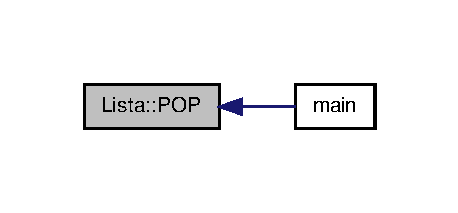
\includegraphics[width=220pt]{class_lista_aba90f4f62ac00f38ecf71ba3c9f1b40e_icgraph}
\end{center}
\end{figure}


\hypertarget{class_lista_a6d81ca560734ac6fce5c503090b7b250}{
\index{Lista@{Lista}!Powiekszenie\_\-Pamieci@{Powiekszenie\_\-Pamieci}}
\index{Powiekszenie\_\-Pamieci@{Powiekszenie\_\-Pamieci}!Lista@{Lista}}
\subsubsection[{Powiekszenie\_\-Pamieci}]{\setlength{\rightskip}{0pt plus 5cm}template$<$typename TYP$>$ void {\bf Lista}$<$ TYP $>$::Powiekszenie\_\-Pamieci (
\begin{DoxyParamCaption}
{}
\end{DoxyParamCaption}
)\hspace{0.3cm}{\ttfamily  \mbox{[}inline\mbox{]}}}}
\label{class_lista_a6d81ca560734ac6fce5c503090b7b250}


Definicja w linii 63 pliku Lista.hh.

\hypertarget{class_lista_a5c21bab22b627c729ad0c90e1f835901}{
\index{Lista@{Lista}!PUSH@{PUSH}}
\index{PUSH@{PUSH}!Lista@{Lista}}
\subsubsection[{PUSH}]{\setlength{\rightskip}{0pt plus 5cm}template$<$typename TYP$>$ void {\bf Lista}$<$ TYP $>$::PUSH (
\begin{DoxyParamCaption}
\item[{TYP}]{ liczba}
\end{DoxyParamCaption}
)\hspace{0.3cm}{\ttfamily  \mbox{[}inline\mbox{]}}}}
\label{class_lista_a5c21bab22b627c729ad0c90e1f835901}


Reimplementowana w \hyperlink{class_kolejka_a66056e67a0514466d7771da351e8468b}{Kolejka$<$ TYP $>$} i \hyperlink{class_stos_a773cf22cb5c67bda0d2878a1ec8bc363}{Stos$<$ TYP $>$}.



Definicja w linii 47 pliku Lista.hh.



Oto graf wywoływań tej funkcji:
\nopagebreak
\begin{figure}[H]
\begin{center}
\leavevmode
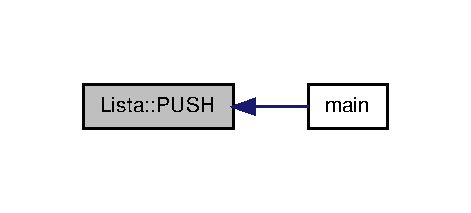
\includegraphics[width=226pt]{class_lista_a5c21bab22b627c729ad0c90e1f835901_icgraph}
\end{center}
\end{figure}


\hypertarget{class_lista_a81ea74ac702b5ccbe3c88b3149887975}{
\index{Lista@{Lista}!Rozmiar@{Rozmiar}}
\index{Rozmiar@{Rozmiar}!Lista@{Lista}}
\subsubsection[{Rozmiar}]{\setlength{\rightskip}{0pt plus 5cm}template$<$typename TYP$>$ void {\bf Lista}$<$ TYP $>$::Rozmiar (
\begin{DoxyParamCaption}
{}
\end{DoxyParamCaption}
)\hspace{0.3cm}{\ttfamily  \mbox{[}inline\mbox{]}}}}
\label{class_lista_a81ea74ac702b5ccbe3c88b3149887975}


Definicja w linii 36 pliku Lista.hh.



Oto graf wywoływań tej funkcji:
\nopagebreak
\begin{figure}[H]
\begin{center}
\leavevmode
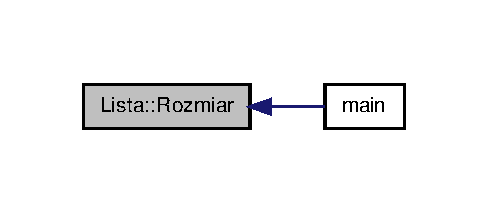
\includegraphics[width=234pt]{class_lista_a81ea74ac702b5ccbe3c88b3149887975_icgraph}
\end{center}
\end{figure}


\hypertarget{class_lista_a89bbb449a047593eebce602a449ac1e7}{
\index{Lista@{Lista}!SHOW@{SHOW}}
\index{SHOW@{SHOW}!Lista@{Lista}}
\subsubsection[{SHOW}]{\setlength{\rightskip}{0pt plus 5cm}template$<$typename TYP$>$ void {\bf Lista}$<$ TYP $>$::SHOW (
\begin{DoxyParamCaption}
{}
\end{DoxyParamCaption}
)\hspace{0.3cm}{\ttfamily  \mbox{[}inline\mbox{]}}}}
\label{class_lista_a89bbb449a047593eebce602a449ac1e7}


Reimplementowana w \hyperlink{class_kolejka_a26b5afbcc9f892a41acbd3aed062ee50}{Kolejka$<$ TYP $>$} i \hyperlink{class_stos_a8f1c40b779a699c84b20eeb59ca67f06}{Stos$<$ TYP $>$}.



Definicja w linii 123 pliku Lista.hh.



Oto graf wywoływań tej funkcji:
\nopagebreak
\begin{figure}[H]
\begin{center}
\leavevmode
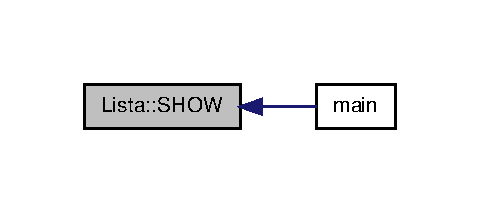
\includegraphics[width=230pt]{class_lista_a89bbb449a047593eebce602a449ac1e7_icgraph}
\end{center}
\end{figure}


\hypertarget{class_lista_a4f10ca015c6b34a322dbc1c93e313c07}{
\index{Lista@{Lista}!SIZE@{SIZE}}
\index{SIZE@{SIZE}!Lista@{Lista}}
\subsubsection[{SIZE}]{\setlength{\rightskip}{0pt plus 5cm}template$<$typename TYP$>$ unsigned int {\bf Lista}$<$ TYP $>$::SIZE (
\begin{DoxyParamCaption}
{}
\end{DoxyParamCaption}
)\hspace{0.3cm}{\ttfamily  \mbox{[}inline\mbox{]}}}}
\label{class_lista_a4f10ca015c6b34a322dbc1c93e313c07}


Reimplementowana w \hyperlink{class_kolejka_a06a7fe157ff434771a700ffd084dc7a2}{Kolejka$<$ TYP $>$} i \hyperlink{class_stos_a6ff0d2aa5946c0dc413e3236ca99fd26}{Stos$<$ TYP $>$}.



Definicja w linii 112 pliku Lista.hh.



Oto graf wywoływań tej funkcji:
\nopagebreak
\begin{figure}[H]
\begin{center}
\leavevmode
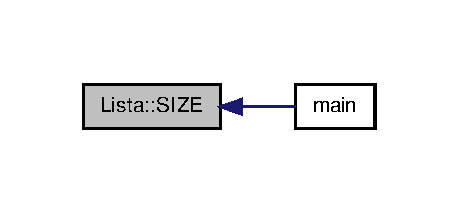
\includegraphics[width=220pt]{class_lista_a4f10ca015c6b34a322dbc1c93e313c07_icgraph}
\end{center}
\end{figure}


\hypertarget{class_lista_aa648e807e5daab59523ffbef5ca80d00}{
\index{Lista@{Lista}!Zmniejszenie\_\-Pamieci@{Zmniejszenie\_\-Pamieci}}
\index{Zmniejszenie\_\-Pamieci@{Zmniejszenie\_\-Pamieci}!Lista@{Lista}}
\subsubsection[{Zmniejszenie\_\-Pamieci}]{\setlength{\rightskip}{0pt plus 5cm}template$<$typename TYP$>$ void {\bf Lista}$<$ TYP $>$::Zmniejszenie\_\-Pamieci (
\begin{DoxyParamCaption}
{}
\end{DoxyParamCaption}
)\hspace{0.3cm}{\ttfamily  \mbox{[}inline\mbox{]}}}}
\label{class_lista_aa648e807e5daab59523ffbef5ca80d00}


Definicja w linii 71 pliku Lista.hh.



\subsection{Dokumentacja atrybutów składowych}
\hypertarget{class_lista_a5d80dd57d8de81690e58a9ee0e33fb68}{
\index{Lista@{Lista}!\_\-rozmiar\_\-listy@{\_\-rozmiar\_\-listy}}
\index{\_\-rozmiar\_\-listy@{\_\-rozmiar\_\-listy}!Lista@{Lista}}
\subsubsection[{\_\-rozmiar\_\-listy}]{\setlength{\rightskip}{0pt plus 5cm}template$<$typename TYP$>$ unsigned int {\bf Lista}$<$ TYP $>$::{\bf \_\-rozmiar\_\-listy}\hspace{0.3cm}{\ttfamily  \mbox{[}private\mbox{]}}}}
\label{class_lista_a5d80dd57d8de81690e58a9ee0e33fb68}


Definicja w linii 31 pliku Lista.hh.

\hypertarget{class_lista_a086812fe74019e8334883d695f4e6389}{
\index{Lista@{Lista}!koniec@{koniec}}
\index{koniec@{koniec}!Lista@{Lista}}
\subsubsection[{koniec}]{\setlength{\rightskip}{0pt plus 5cm}template$<$typename TYP$>$ unsigned int {\bf Lista}$<$ TYP $>$::{\bf koniec}\hspace{0.3cm}{\ttfamily  \mbox{[}private\mbox{]}}}}
\label{class_lista_a086812fe74019e8334883d695f4e6389}


Definicja w linii 33 pliku Lista.hh.

\hypertarget{class_lista_af6df56635655f71b73c6909032f78f57}{
\index{Lista@{Lista}!poczatek@{poczatek}}
\index{poczatek@{poczatek}!Lista@{Lista}}
\subsubsection[{poczatek}]{\setlength{\rightskip}{0pt plus 5cm}template$<$typename TYP$>$ unsigned int {\bf Lista}$<$ TYP $>$::{\bf poczatek}\hspace{0.3cm}{\ttfamily  \mbox{[}private\mbox{]}}}}
\label{class_lista_af6df56635655f71b73c6909032f78f57}


Definicja w linii 32 pliku Lista.hh.

\hypertarget{class_lista_afdd41700bc843ab4aeb58425b63e4390}{
\index{Lista@{Lista}!tab@{tab}}
\index{tab@{tab}!Lista@{Lista}}
\subsubsection[{tab}]{\setlength{\rightskip}{0pt plus 5cm}template$<$typename TYP$>$ TYP$\ast$ {\bf Lista}$<$ TYP $>$::{\bf tab}\hspace{0.3cm}{\ttfamily  \mbox{[}private\mbox{]}}}}
\label{class_lista_afdd41700bc843ab4aeb58425b63e4390}


Definicja w linii 30 pliku Lista.hh.



Dokumentacja dla tej klasy została wygenerowana z pliku:\begin{DoxyCompactItemize}
\item 
\hyperlink{_lista_8hh}{Lista.hh}\end{DoxyCompactItemize}

\hypertarget{class_stos}{
\section{Dokumentacja szablonu klasy Stos$<$ TYP $>$}
\label{class_stos}\index{Stos@{Stos}}
}


Klasa \hyperlink{class_stos}{Stos}.  




{\ttfamily \#include $<$Stos.hh$>$}



Diagram dziedziczenia dla Stos$<$ TYP $>$
\nopagebreak
\begin{figure}[H]
\begin{center}
\leavevmode
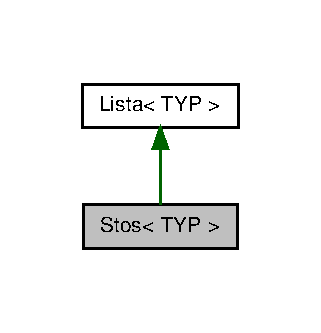
\includegraphics[width=154pt]{class_stos__inherit__graph}
\end{center}
\end{figure}


Diagram współpracy dla Stos$<$ TYP $>$:
\nopagebreak
\begin{figure}[H]
\begin{center}
\leavevmode
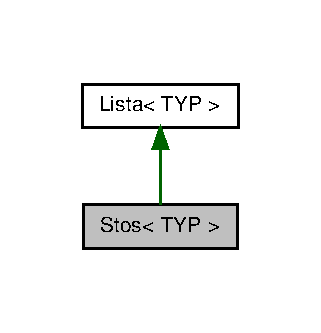
\includegraphics[width=154pt]{class_stos__coll__graph}
\end{center}
\end{figure}
\subsection*{Metody publiczne}
\begin{DoxyCompactItemize}
\item 
void \hyperlink{class_stos_a773cf22cb5c67bda0d2878a1ec8bc363}{PUSH} (TYP liczba)
\item 
int \hyperlink{class_stos_ab8b0ecec7cbe0ae761bfee9d9e47d5d4}{POP} ()
\item 
void \hyperlink{class_stos_a8f1c40b779a699c84b20eeb59ca67f06}{SHOW} ()
\item 
unsigned int \hyperlink{class_stos_a6ff0d2aa5946c0dc413e3236ca99fd26}{SIZE} ()
\end{DoxyCompactItemize}


\subsection{Opis szczegółowy}
\subsubsection*{template$<$typename TYP$>$ class Stos$<$ TYP $>$}

Klasa ta modeluje nam \hyperlink{class_stos}{Stos} Składa się z pól klasy \hyperlink{class_lista}{Lista} (poczatek) ktore zostanie uzyta aby pokazywalo na ostatni element stosu oraz metod PUSH, POP, SIZE, SHOW 

Definicja w linii 25 pliku Stos.hh.



\subsection{Dokumentacja funkcji składowych}
\hypertarget{class_stos_ab8b0ecec7cbe0ae761bfee9d9e47d5d4}{
\index{Stos@{Stos}!POP@{POP}}
\index{POP@{POP}!Stos@{Stos}}
\subsubsection[{POP}]{\setlength{\rightskip}{0pt plus 5cm}template$<$typename TYP$>$ int {\bf Stos}$<$ TYP $>$::POP (
\begin{DoxyParamCaption}
{}
\end{DoxyParamCaption}
)\hspace{0.3cm}{\ttfamily  \mbox{[}inline\mbox{]}}}}
\label{class_stos_ab8b0ecec7cbe0ae761bfee9d9e47d5d4}


Definicja w linii 50 pliku Stos.hh.



Oto graf wywoływań tej funkcji:
\nopagebreak
\begin{figure}[H]
\begin{center}
\leavevmode
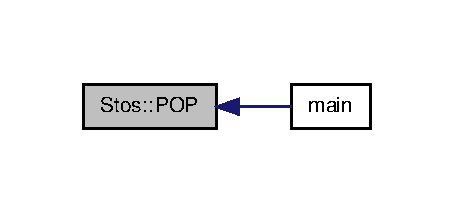
\includegraphics[width=218pt]{class_stos_ab8b0ecec7cbe0ae761bfee9d9e47d5d4_icgraph}
\end{center}
\end{figure}


\hypertarget{class_stos_a773cf22cb5c67bda0d2878a1ec8bc363}{
\index{Stos@{Stos}!PUSH@{PUSH}}
\index{PUSH@{PUSH}!Stos@{Stos}}
\subsubsection[{PUSH}]{\setlength{\rightskip}{0pt plus 5cm}template$<$typename TYP$>$ void {\bf Stos}$<$ TYP $>$::PUSH (
\begin{DoxyParamCaption}
\item[{TYP}]{ liczba}
\end{DoxyParamCaption}
)\hspace{0.3cm}{\ttfamily  \mbox{[}inline\mbox{]}}}}
\label{class_stos_a773cf22cb5c67bda0d2878a1ec8bc363}


Reimplementowana z \hyperlink{class_lista_a5c21bab22b627c729ad0c90e1f835901}{Lista$<$ TYP $>$}.



Definicja w linii 37 pliku Stos.hh.



Oto graf wywoływań tej funkcji:
\nopagebreak
\begin{figure}[H]
\begin{center}
\leavevmode
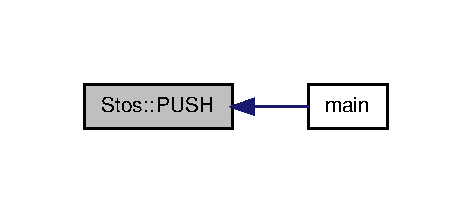
\includegraphics[width=226pt]{class_stos_a773cf22cb5c67bda0d2878a1ec8bc363_icgraph}
\end{center}
\end{figure}


\hypertarget{class_stos_a8f1c40b779a699c84b20eeb59ca67f06}{
\index{Stos@{Stos}!SHOW@{SHOW}}
\index{SHOW@{SHOW}!Stos@{Stos}}
\subsubsection[{SHOW}]{\setlength{\rightskip}{0pt plus 5cm}template$<$typename TYP$>$ void {\bf Stos}$<$ TYP $>$::SHOW (
\begin{DoxyParamCaption}
{}
\end{DoxyParamCaption}
)\hspace{0.3cm}{\ttfamily  \mbox{[}inline\mbox{]}}}}
\label{class_stos_a8f1c40b779a699c84b20eeb59ca67f06}


Reimplementowana z \hyperlink{class_lista_a89bbb449a047593eebce602a449ac1e7}{Lista$<$ TYP $>$}.



Definicja w linii 58 pliku Stos.hh.



Oto graf wywoływań tej funkcji:
\nopagebreak
\begin{figure}[H]
\begin{center}
\leavevmode
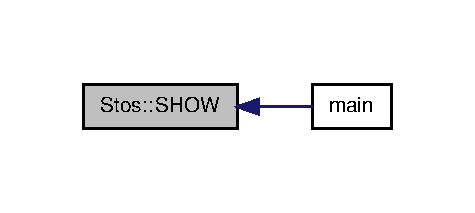
\includegraphics[width=228pt]{class_stos_a8f1c40b779a699c84b20eeb59ca67f06_icgraph}
\end{center}
\end{figure}


\hypertarget{class_stos_a6ff0d2aa5946c0dc413e3236ca99fd26}{
\index{Stos@{Stos}!SIZE@{SIZE}}
\index{SIZE@{SIZE}!Stos@{Stos}}
\subsubsection[{SIZE}]{\setlength{\rightskip}{0pt plus 5cm}template$<$typename TYP$>$ unsigned int {\bf Stos}$<$ TYP $>$::SIZE (
\begin{DoxyParamCaption}
{}
\end{DoxyParamCaption}
)\hspace{0.3cm}{\ttfamily  \mbox{[}inline\mbox{]}}}}
\label{class_stos_a6ff0d2aa5946c0dc413e3236ca99fd26}


Reimplementowana z \hyperlink{class_lista_a4f10ca015c6b34a322dbc1c93e313c07}{Lista$<$ TYP $>$}.



Definicja w linii 67 pliku Stos.hh.



Dokumentacja dla tej klasy została wygenerowana z pliku:\begin{DoxyCompactItemize}
\item 
\hyperlink{_stos_8hh}{Stos.hh}\end{DoxyCompactItemize}

\chapter{Dokumentacja plików}
\hypertarget{_benchmark_8cpp}{
\section{Dokumentacja pliku Benchmark.cpp}
\label{_benchmark_8cpp}\index{Benchmark.cpp@{Benchmark.cpp}}
}


Metody klasy \hyperlink{class_benchmark}{Benchmark}.  


{\ttfamily \#include \char`\"{}Benchmark.hh\char`\"{}}\par
{\ttfamily \#include $<$cstdlib$>$}\par
{\ttfamily \#include $<$fstream$>$}\par
{\ttfamily \#include $<$ctime$>$}\par
Wykres zależności załączania dla Benchmark.cpp:
\nopagebreak
\begin{figure}[H]
\begin{center}
\leavevmode
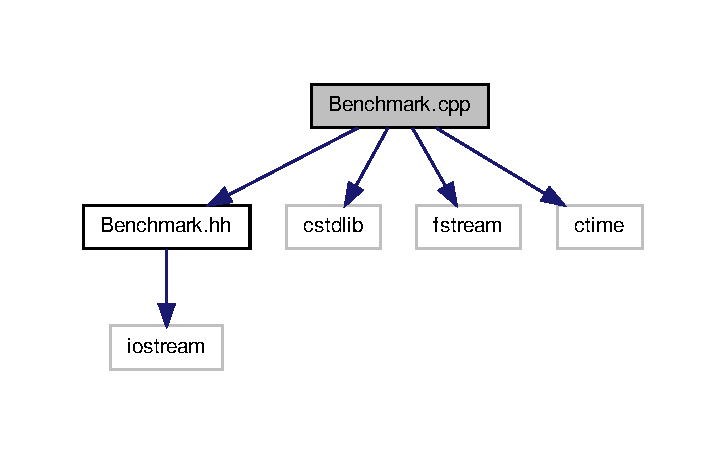
\includegraphics[width=348pt]{_benchmark_8cpp__incl}
\end{center}
\end{figure}


\subsection{Opis szczegółowy}
Plik zawiera definicje metod klasy \hyperlink{class_benchmark}{Benchmark} 

Definicja w pliku \hyperlink{_benchmark_8cpp_source}{Benchmark.cpp}.


\hypertarget{_benchmark_8hh}{
\section{Dokumentacja pliku Benchmark.hh}
\label{_benchmark_8hh}\index{Benchmark.hh@{Benchmark.hh}}
}


Definicja klasy \hyperlink{class_benchmark}{Benchmark}.  


{\ttfamily \#include $<$iostream$>$}\par
Wykres zależności załączania dla Benchmark.hh:
\nopagebreak
\begin{figure}[H]
\begin{center}
\leavevmode
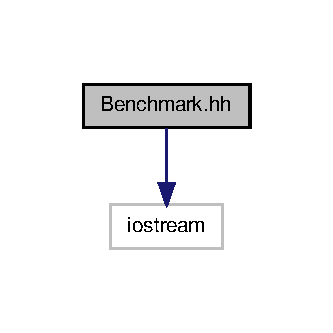
\includegraphics[width=160pt]{_benchmark_8hh__incl}
\end{center}
\end{figure}
Ten wykres pokazuje, które pliki bezpośrednio lub pośrednio załączają ten plik:
\nopagebreak
\begin{figure}[H]
\begin{center}
\leavevmode
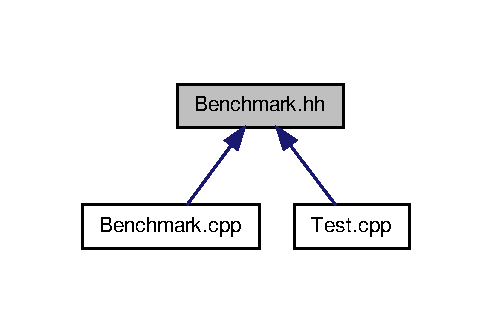
\includegraphics[width=238pt]{_benchmark_8hh__dep__incl}
\end{center}
\end{figure}
\subsection*{Komponenty}
\begin{DoxyCompactItemize}
\item 
class \hyperlink{class_benchmark}{Benchmark}
\begin{DoxyCompactList}\small\item\em Klasa \hyperlink{class_benchmark}{Benchmark}. \item\end{DoxyCompactList}\end{DoxyCompactItemize}


\subsection{Opis szczegółowy}
Plik zawiera definicje klasy \hyperlink{class_benchmark}{Benchmark} ktora bedzie wyznaczala nam punkty do wyznaczenia zlozonosci obliczeniowej. 

Definicja w pliku \hyperlink{_benchmark_8hh_source}{Benchmark.hh}.


\hypertarget{_kolejka_8hh}{
\section{Dokumentacja pliku Kolejka.hh}
\label{_kolejka_8hh}\index{Kolejka.hh@{Kolejka.hh}}
}


Definicja klasy \hyperlink{class_kolejka}{Kolejka}.  


{\ttfamily \#include $<$iostream$>$}\par
{\ttfamily \#include \char`\"{}Lista.hh\char`\"{}}\par
Wykres zależności załączania dla Kolejka.hh:
\nopagebreak
\begin{figure}[H]
\begin{center}
\leavevmode
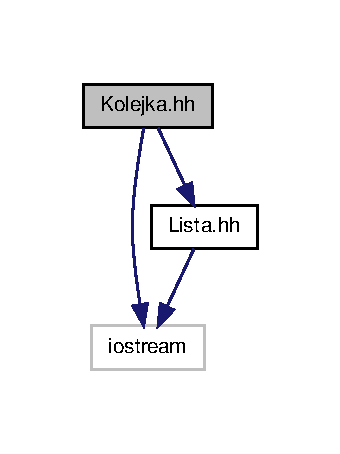
\includegraphics[width=163pt]{_kolejka_8hh__incl}
\end{center}
\end{figure}
Ten wykres pokazuje, które pliki bezpośrednio lub pośrednio załączają ten plik:
\nopagebreak
\begin{figure}[H]
\begin{center}
\leavevmode
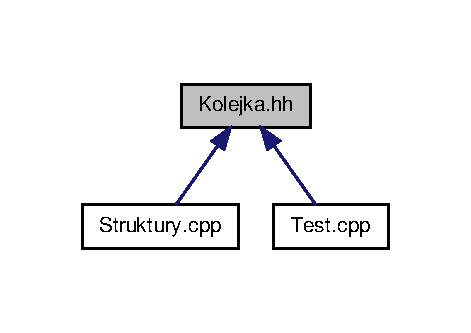
\includegraphics[width=226pt]{_kolejka_8hh__dep__incl}
\end{center}
\end{figure}
\subsection*{Komponenty}
\begin{DoxyCompactItemize}
\item 
class \hyperlink{class_kolejka}{Kolejka$<$ TYP $>$}
\begin{DoxyCompactList}\small\item\em Klasa \hyperlink{class_kolejka}{Kolejka}. \item\end{DoxyCompactList}\end{DoxyCompactItemize}


\subsection{Opis szczegółowy}
Plik zawiera definicje klasy \hyperlink{class_kolejka}{Kolejka}, ktora bedzie struktura naszych danych. Klasa ta posiada szablon, dzieki czemu mozemy pracowac na roznych typach danych 

Definicja w pliku \hyperlink{_kolejka_8hh_source}{Kolejka.hh}.


\hypertarget{_lista_8cpp}{
\section{Dokumentacja pliku Lista.cpp}
\label{_lista_8cpp}\index{Lista.cpp@{Lista.cpp}}
}
{\ttfamily \#include $<$iostream$>$}\par
{\ttfamily \#include \char`\"{}Lista.hh\char`\"{}}\par
Wykres zależności załączania dla Lista.cpp:
\nopagebreak
\begin{figure}[H]
\begin{center}
\leavevmode
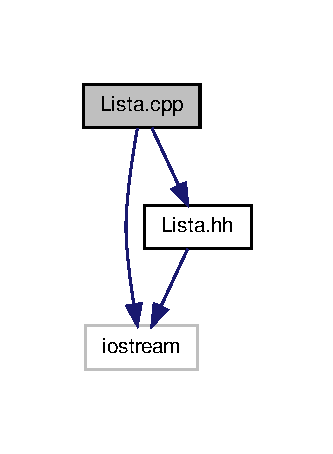
\includegraphics[width=160pt]{_lista_8cpp__incl}
\end{center}
\end{figure}
\subsection*{Funkcje}
\begin{DoxyCompactItemize}
\item 
int \hyperlink{_lista_8cpp_ae66f6b31b5ad750f1fe042a706a4e3d4}{main} ()
\end{DoxyCompactItemize}


\subsection{Dokumentacja funkcji}
\hypertarget{_lista_8cpp_ae66f6b31b5ad750f1fe042a706a4e3d4}{
\index{Lista.cpp@{Lista.cpp}!main@{main}}
\index{main@{main}!Lista.cpp@{Lista.cpp}}
\subsubsection[{main}]{\setlength{\rightskip}{0pt plus 5cm}int main (
\begin{DoxyParamCaption}
{}
\end{DoxyParamCaption}
)}}
\label{_lista_8cpp_ae66f6b31b5ad750f1fe042a706a4e3d4}


Definicja w linii 6 pliku Lista.cpp.



Oto graf wywołań dla tej funkcji:
\nopagebreak
\begin{figure}[H]
\begin{center}
\leavevmode
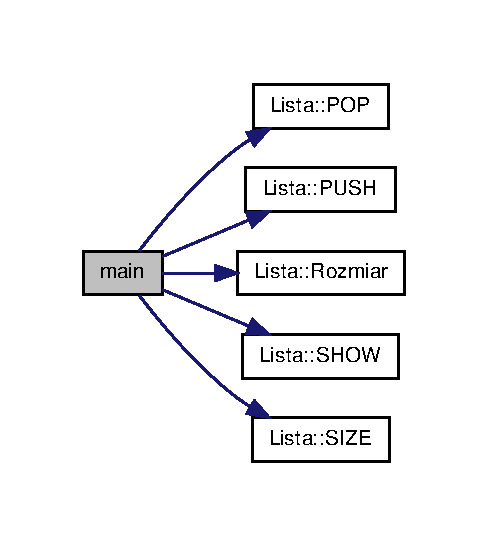
\includegraphics[width=234pt]{_lista_8cpp_ae66f6b31b5ad750f1fe042a706a4e3d4_cgraph}
\end{center}
\end{figure}



\hypertarget{_lista_8hh}{
\section{Dokumentacja pliku Lista.hh}
\label{_lista_8hh}\index{Lista.hh@{Lista.hh}}
}


Definicja klasy \hyperlink{class_lista}{Lista}.  


{\ttfamily \#include $<$iostream$>$}\par
{\ttfamily \#include \char`\"{}Element.hh\char`\"{}}\par
Wykres zależności załączania dla Lista.hh:
\nopagebreak
\begin{figure}[H]
\begin{center}
\leavevmode
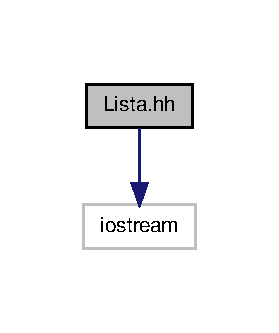
\includegraphics[width=218pt]{_lista_8hh__incl}
\end{center}
\end{figure}
Ten wykres pokazuje, które pliki bezpośrednio lub pośrednio załączają ten plik:
\nopagebreak
\begin{figure}[H]
\begin{center}
\leavevmode
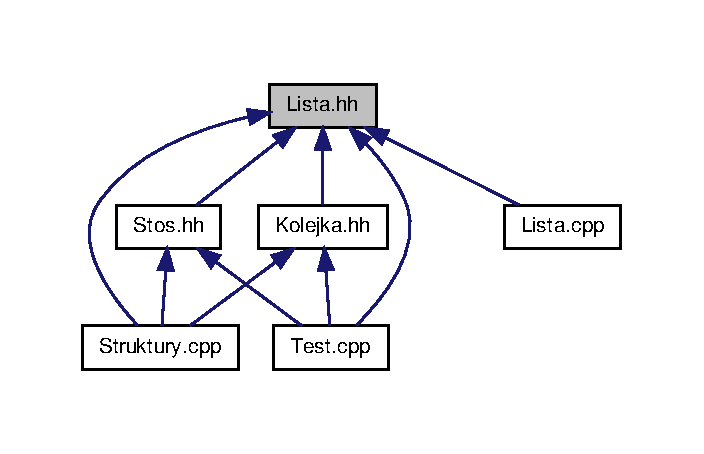
\includegraphics[width=235pt]{_lista_8hh__dep__incl}
\end{center}
\end{figure}
\subsection*{Komponenty}
\begin{DoxyCompactItemize}
\item 
class \hyperlink{class_lista}{Lista$<$ TYP $>$}
\begin{DoxyCompactList}\small\item\em Klasa \hyperlink{class_lista}{Lista}. \item\end{DoxyCompactList}\end{DoxyCompactItemize}


\subsection{Opis szczegółowy}
Plik zawiera definicje klasy \hyperlink{class_lista}{Lista}, ktora bedzie struktura naszych danych. Klasa ta posiada szablon, dzieki czemu mozemy pracowac na roznych typach danych 

Definicja w pliku \hyperlink{_lista_8hh_source}{Lista.hh}.


\hypertarget{_stos_8hh}{
\section{Dokumentacja pliku Stos.hh}
\label{_stos_8hh}\index{Stos.hh@{Stos.hh}}
}


Definicja klasy \hyperlink{class_stos}{Stos}.  


{\ttfamily \#include $<$iostream$>$}\par
{\ttfamily \#include \char`\"{}Lista.hh\char`\"{}}\par
Wykres zależności załączania dla Stos.hh:
\nopagebreak
\begin{figure}[H]
\begin{center}
\leavevmode
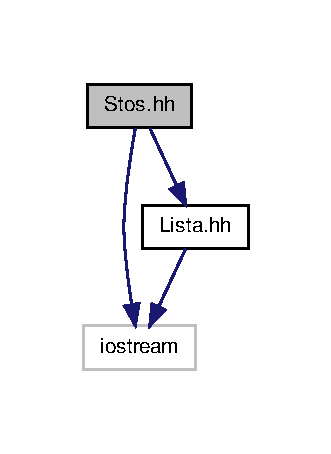
\includegraphics[width=159pt]{_stos_8hh__incl}
\end{center}
\end{figure}
Ten wykres pokazuje, które pliki bezpośrednio lub pośrednio załączają ten plik:
\nopagebreak
\begin{figure}[H]
\begin{center}
\leavevmode
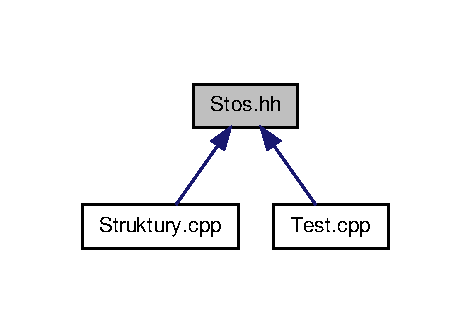
\includegraphics[width=226pt]{_stos_8hh__dep__incl}
\end{center}
\end{figure}
\subsection*{Komponenty}
\begin{DoxyCompactItemize}
\item 
class \hyperlink{class_stos}{Stos$<$ TYP $>$}
\begin{DoxyCompactList}\small\item\em Klasa \hyperlink{class_stos}{Stos}. \item\end{DoxyCompactList}\end{DoxyCompactItemize}


\subsection{Opis szczegółowy}
Plik zawiera definicje klasy \hyperlink{class_stos}{Stos}, ktora bedzie struktura naszych danych. Klasa ta posiada szablon, dzieki czemu mozemy pracowac na roznych typach danych 

Definicja w pliku \hyperlink{_stos_8hh_source}{Stos.hh}.


\hypertarget{strona_8dox}{
\section{Dokumentacja pliku strona.dox}
\label{strona_8dox}\index{strona.dox@{strona.dox}}
}

\hypertarget{_struktury_8cpp}{
\section{Dokumentacja pliku Struktury.cpp}
\label{_struktury_8cpp}\index{Struktury.cpp@{Struktury.cpp}}
}
{\ttfamily \#include $<$iostream$>$}\par
{\ttfamily \#include \char`\"{}Lista.hh\char`\"{}}\par
{\ttfamily \#include \char`\"{}Kolejka.hh\char`\"{}}\par
{\ttfamily \#include \char`\"{}Stos.hh\char`\"{}}\par
Wykres zależności załączania dla Struktury.cpp:
\nopagebreak
\begin{figure}[H]
\begin{center}
\leavevmode
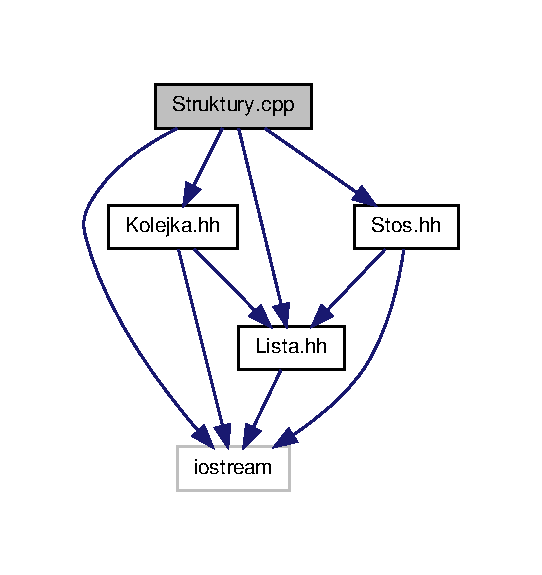
\includegraphics[width=260pt]{_struktury_8cpp__incl}
\end{center}
\end{figure}
\subsection*{Funkcje}
\begin{DoxyCompactItemize}
\item 
int \hyperlink{_struktury_8cpp_ae66f6b31b5ad750f1fe042a706a4e3d4}{main} ()
\end{DoxyCompactItemize}


\subsection{Dokumentacja funkcji}
\hypertarget{_struktury_8cpp_ae66f6b31b5ad750f1fe042a706a4e3d4}{
\index{Struktury.cpp@{Struktury.cpp}!main@{main}}
\index{main@{main}!Struktury.cpp@{Struktury.cpp}}
\subsubsection[{main}]{\setlength{\rightskip}{0pt plus 5cm}int main (
\begin{DoxyParamCaption}
{}
\end{DoxyParamCaption}
)}}
\label{_struktury_8cpp_ae66f6b31b5ad750f1fe042a706a4e3d4}


Definicja w linii 8 pliku Struktury.cpp.



Oto graf wywołań dla tej funkcji:
\nopagebreak
\begin{figure}[H]
\begin{center}
\leavevmode
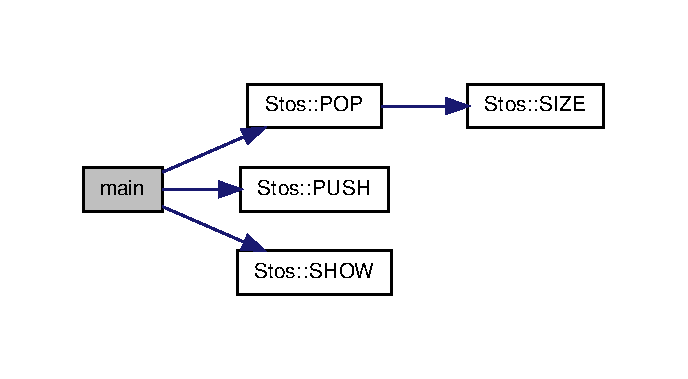
\includegraphics[width=330pt]{_struktury_8cpp_ae66f6b31b5ad750f1fe042a706a4e3d4_cgraph}
\end{center}
\end{figure}



\hypertarget{_test_8cpp}{
\section{Dokumentacja pliku Test.cpp}
\label{_test_8cpp}\index{Test.cpp@{Test.cpp}}
}
{\ttfamily \#include $<$iostream$>$}\par
{\ttfamily \#include \char`\"{}Benchmark.hh\char`\"{}}\par
{\ttfamily \#include \char`\"{}Lista.hh\char`\"{}}\par
{\ttfamily \#include \char`\"{}Kolejka.hh\char`\"{}}\par
{\ttfamily \#include \char`\"{}Stos.hh\char`\"{}}\par
Wykres zależności załączania dla Test.cpp:
\nopagebreak
\begin{figure}[H]
\begin{center}
\leavevmode
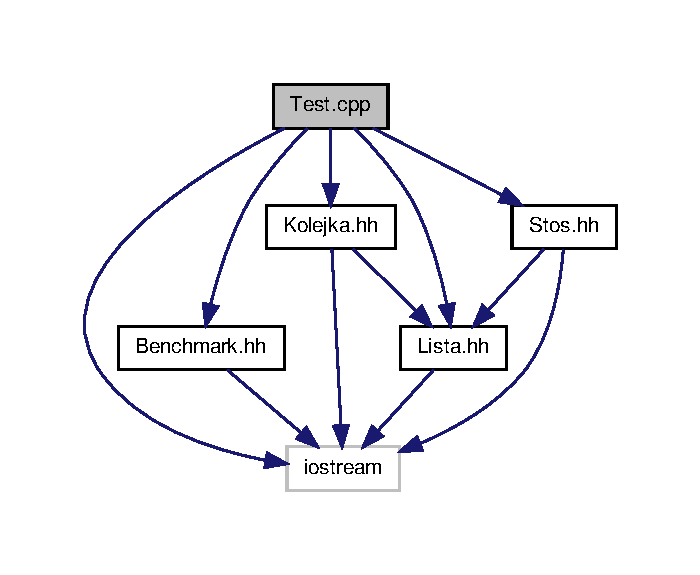
\includegraphics[width=336pt]{_test_8cpp__incl}
\end{center}
\end{figure}
\subsection*{Definicje}
\begin{DoxyCompactItemize}
\item 
\#define \hyperlink{_test_8cpp_a77b984cfb88c2ca29fea115a7019ba8f}{STALA}~10
\end{DoxyCompactItemize}
\subsection*{Funkcje}
\begin{DoxyCompactItemize}
\item 
double \hyperlink{_test_8cpp_ae36bd4cd4ba4a0663e79b579bf31fc20}{funkcja} (double x)
\item 
int \hyperlink{_test_8cpp_ae66f6b31b5ad750f1fe042a706a4e3d4}{main} ()
\end{DoxyCompactItemize}


\subsection{Dokumentacja definicji}
\hypertarget{_test_8cpp_a77b984cfb88c2ca29fea115a7019ba8f}{
\index{Test.cpp@{Test.cpp}!STALA@{STALA}}
\index{STALA@{STALA}!Test.cpp@{Test.cpp}}
\subsubsection[{STALA}]{\setlength{\rightskip}{0pt plus 5cm}\#define STALA~10}}
\label{_test_8cpp_a77b984cfb88c2ca29fea115a7019ba8f}


Definicja w linii 7 pliku Test.cpp.



\subsection{Dokumentacja funkcji}
\hypertarget{_test_8cpp_ae36bd4cd4ba4a0663e79b579bf31fc20}{
\index{Test.cpp@{Test.cpp}!funkcja@{funkcja}}
\index{funkcja@{funkcja}!Test.cpp@{Test.cpp}}
\subsubsection[{funkcja}]{\setlength{\rightskip}{0pt plus 5cm}double funkcja (
\begin{DoxyParamCaption}
\item[{double}]{ x}
\end{DoxyParamCaption}
)}}
\label{_test_8cpp_ae36bd4cd4ba4a0663e79b579bf31fc20}


Definicja w linii 10 pliku Test.cpp.

\hypertarget{_test_8cpp_ae66f6b31b5ad750f1fe042a706a4e3d4}{
\index{Test.cpp@{Test.cpp}!main@{main}}
\index{main@{main}!Test.cpp@{Test.cpp}}
\subsubsection[{main}]{\setlength{\rightskip}{0pt plus 5cm}int main (
\begin{DoxyParamCaption}
{}
\end{DoxyParamCaption}
)}}
\label{_test_8cpp_ae66f6b31b5ad750f1fe042a706a4e3d4}


Definicja w linii 14 pliku Test.cpp.



Oto graf wywołań dla tej funkcji:
\nopagebreak
\begin{figure}[H]
\begin{center}
\leavevmode
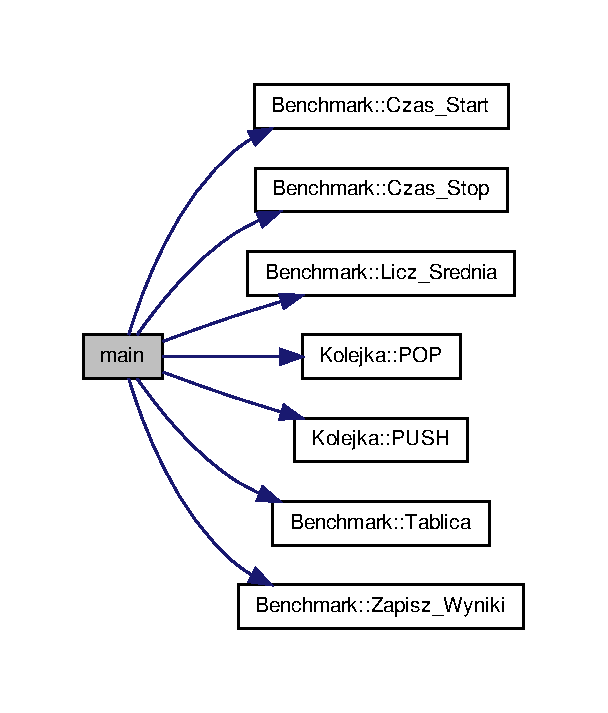
\includegraphics[width=292pt]{_test_8cpp_ae66f6b31b5ad750f1fe042a706a4e3d4_cgraph}
\end{center}
\end{figure}



\printindex
\end{document}
